%
% speed_of_sound.tex - Final Project LaTeX file
%
% 01Aug17  Jackson Sheppard
%
\documentclass[12pt]{article}
\usepackage{fancyhdr}
\usepackage{graphicx}
\usepackage{color}
\usepackage{hyperref}
\usepackage{indentfirst}
\pagenumbering{arabic}

% Uncomment one of the following lines to use Times-Roman and Helvetica
% or Palatino instead of Computer Modern.
% \usepackage{txfonts}
% \usepackage[sc]{mathpazo}\linespread{1.05}\usepackage[scaled]{helvet}

\usepackage[hmargin=90bp,tmargin=108bp,bmargin=72bp,
            headheight=15bp,footskip=40bp]{geometry}
%%%%%%%%%%%%%%%%%%%%%%%%%%%%%%%%%%%%%%%%%%%%%%%%%%%%%%%%%%%%%%%%%%%%%%%%%%%%%%%

%
% custom definitions
%
\newcommand\thisis{Measurement of the speed of sound in air}
\newcommand\theauthor{Jackson~Sheppard}

\newcommand\sfb{\sffamily\bfseries}

\newcommand\red[1]{\textcolor{red}{\sffamily\bfseries #1}}
%%%%%%%%%%%%%%%%%%%%%%%%%%%%%%%%%%%%%%%%%%%%%%%%%%%%%%%%%%%%%%%%%%%%%%%%%%%%%%%

%
% custom heading and footer
%
\fancypagestyle{firstpg}
   {
   \fancyhf{}%
   \cfoot{\sffamily\thepage}%
   \renewcommand\headrulewidth{0bp}
   }

\pagestyle{fancy}
\lhead{\sffamily \thisis}
\chead{}
\rhead{\sffamily \theauthor}

\lfoot{}
\cfoot{\sffamily\thepage}
\rfoot{}
%%%%%%%%%%%%%%%%%%%%%%%%%%%%%%%%%%%%%%%%%%%%%%%%%%%%%%%%%%%%%%%%%%%%%%%%%%%%%%%
\begin{document}
\thispagestyle{firstpg}

\noindent
{\sffamily\bfseries\huge \thisis}\\

\noindent
{\large\sffamily \theauthor}\\
\today
\vspace*{20bp}

\noindent
The program "speed\_of\_sound.py" analyzes an audio recording of white
noise played through a speaker at one end of an open-ended tube of known length.
With a microphone placed at the other end, this sound is recorded
and saved as a wave file. The program then performs a Fast Fourier
Transform (FFT) on the data to obtain a spectrogram and the frequencies
of maximum intensity. These resonant frequencies are
then used to calculate the speed of sound. Using a $20$ second audio
clip of white noise played through a tube of length $0.61595$ m, this
program calculated the speed of sound in air to be $326.35$ m/s, having
a relative error of $4.85\%$ from the accepted value.

\section{Installing Necessary Software}
The only necessary external software not already present on the
Raspberry Pi for this class is a tool set called "alsa-utils" that is 
developed for Advanced Linux Sound Architecture (ALSA), a program used 
for recording and waveform editing. This can be installed using the following
command:
\\
\\
sudo apt-get install alsa-utils
\\

The other necessary packages to run this program should already be present upon running the update script for this course, but they include
matplotlib.pyplot, matplotlib.mlab, numpy, scipy.io.wavfile, subprocess,
sys, and time.

\section{Necessary External Hardware}
This program requires the use of a USB microphone to record the audio signal
generated by the white noise. For this experiment, I used the VAlinks(TM) Mini
Flexible Plug and Play Home Studio USB Mic, purchased on amazon:
\url{https://www.amazon.com/VAlinks-Microphone-Recording-Compatible-Raspberry/dp/B014MASID4}. 
This allows for simple recording of audio files and saving them as wave files
using the alsa program. In addition, it requires a white noise generator, which
can be found online at: 
\url{https://mynoise.net/NoiseMachines/whiteNoiseGenerator.php},
along with a speaker to amplify the noise.

\section{Project Description}
This program determines the speed of sound in air by finding the resonant
frequencies of an open-ended tube through fourier transform analysis of an
audio signal.

The set up of this experiment is to place a speaker and microphone on either
end of a tube of known length. The user then plays white noise through
the speaker while the program records the audio clip for a set time limit of
$20$ seconds that has been hard coded into the program. This time scale allows
for optimal accuracy of the transformation.

After either opening the chosen wave file or recording a new sample, the program
stores the sampling frequency in a variable and the audio data in
a $N$ rows by $2$ columns multidimensional array, corresponding to the N frames
in the sample and two channels for stereo input. The entries in the array
correspond to the relative sound level while the indeces are their
frame number. To convert to time in seconds,
the program computes the signal time by dividing the number of frames by the
sampling frequency and then creates an array of time points with the same
number of entries as there are frames and runs from $t=0$ to the signal time.

The transformation to frequency space is simplified if the audio signal
recorded in stereo and stored in an $N$ by $2$ array is downmixed to mono and
stored in a one dimensional array. The program therefore averages the contents
in each channel and stores the result as a new array corresponding to the mono
data. This now one dimensional array is then fourier transformed for frequency
analysis.

After plotting the mono sound level versus time, the program computes a
power spectrum distrubution using the matplotlib.mlab function "psd". This
function is passed as arguments the array containing the mono data, the number
of points to transform, and the sampling rate to be used. The function then
computes a FFT of the input data set, takes the absolute value 
squared of the result, and stores only the data corresponding to positive
frequencies. The function outputs two arrays, the first containing the frequency
spectrum of the signal and the second containing their corresponding
intensities.

Plotting the data produced by the transformation results in a spectrogram with
sharp peaks at the resonant frequencies of the tube. The set of $n$ resonant
frequencies ($n$ harmonics) for an open-ended tube satisfy:
\begin{equation} \label{eq:1}
f_n = \frac{nv}{2L}
\end{equation}

Here, $f_n$ is the $n$'th harmonic frequency, L is the length of the tube, and
v is the speed of sound. Thus, after creating a spectrogram, the program finds
the first four peak frequencies and plots these values against their harmonic
number $n$. It then fits a linear equation to the $f_n$ vs $n$ plot and obtains
the slope for a measurment of the speed of sound in air.

%------------------------------------------------------------------------------
\begin{figure}[h]
\begin{center}
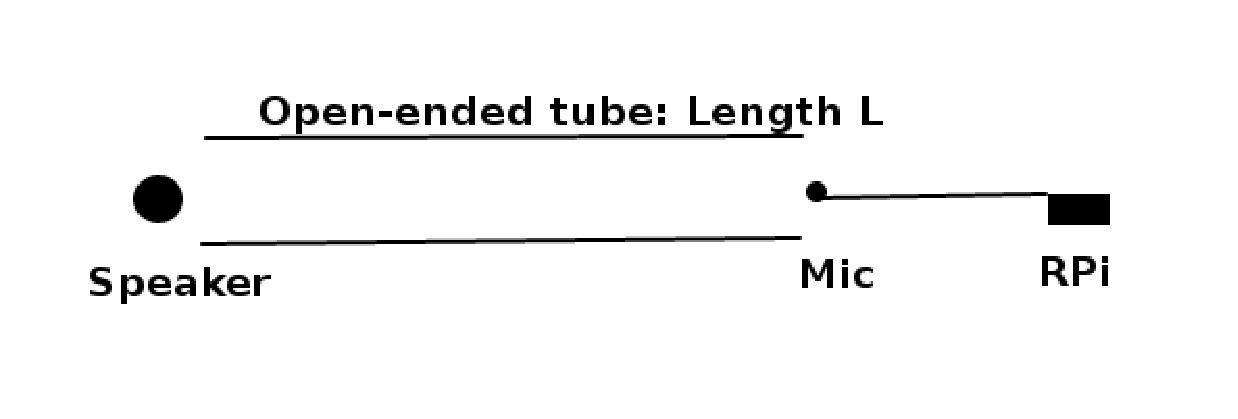
\includegraphics[width=300bp]{exp_setup.eps}
\vspace{-18bp}
\end{center}
\caption[]{\label{fig:setup}\small
Schematic representation of experiment setup. The user should place the speaker 
and microphone at opposite edges of the tube. The microphone should be connected
to the RPi through USB port (1,0), which is the top port directly next to the
ethernet port.
}
\end{figure}
%------------------------------------------------------------------------------

\section{Results}
The set up for this experiment is shown schematically in Fig.~\ref{fig:setup}.
This shows the speaker and microphone placed on either side of the tube and
the microphone connected to the RPi through one of its USB ports. Here the user
of this program should take note of the length of the tube and update the
constant variable "LENGTH" hard coded into the top of the program. However,
for each wave file in the directory containing this program, the length used
was $0.61595$ m and so this value is set in the program. It is also
necessary that the user insert the microphone USB into the RPi USB device port
(1,0), which corresponds to the top USB port directly next to the ethernet
port. This step is necessary for execution because the python program uses
the subprocess function "call" to run the Linux program "arecord" with this
option specifying the USB port. To troubleshoot the microphone or change the
port, the following commands are very useful:
\\
\\
arecord -f dat -d 20 -D plughw:1,0 test.wav\\
\# used to record 20 second audio clip onto new wave file test.wav\\
aplay -f dat test.wav\\
\# used to play back wave file test.wav\\
arecord -l\\
\# show list of CAPTURE Hardware Devices able to record
\\

The above commands are useful primarily for setting up the microphone.
However, if the device is connected to the USB port described
previously, then the python program will capture the audio input from the
device correctly.

After connecting the USB microphone, setting the length of the tube inside
the program code, and positioning the speaker as shown in Fig.~\ref{fig:setup},
the user should run the program and follow the prompt to either enter the name
of a pre-existing wave file saved in the current working directory or record a
new file.

For this results section, the program recorded an audio file with a tube of
length $L = 0.61595$ m that is now saved as "noise2.wav". After the
recording is finished, the program reads the data and determines the
number of frames in the sample and its signal time.
The program then converts the audio sample from stereo to mono by averaging
the data in each channel. It could be more efficent to instead transform the
stereo data, but this would require the psd function to process twice as much
data, and the implementation of this is more complicated.

%------------------------------------------------------------------------------
\begin{figure}[h]
\begin{center}
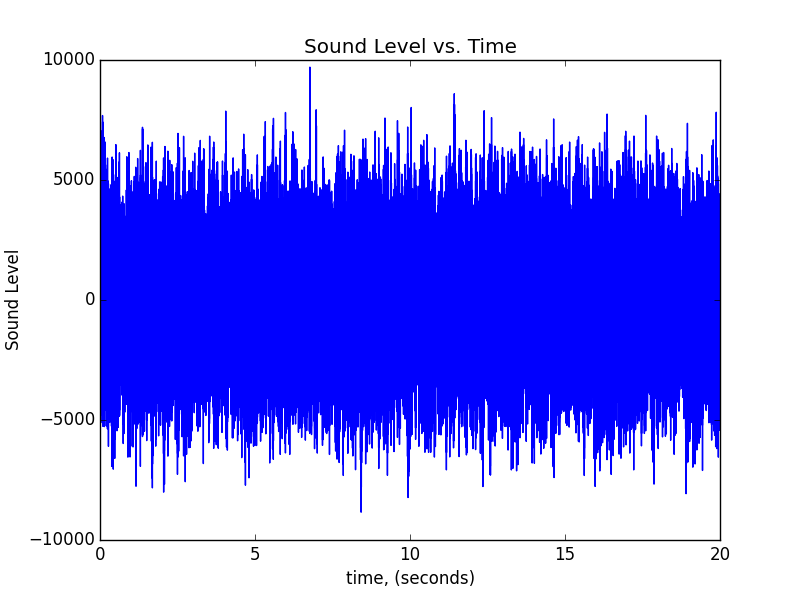
\includegraphics[width=300bp]{noise2_soundvtime.png}
\vspace{-18bp}
\end{center}
\caption[]{\label{fig:soundvtime}\small
Plot of sound level versus time. The sound was captured with a USB microphone 
and plotted using the matplotlib.pyplot library. The units of the time
axis are in seconds while the units of the sound level axis are arbitrary as
we are only interested in relative intensities at specific frequencies.
}
\end{figure}
%------------------------------------------------------------------------------

After converting the signal from stereo to mono, the program plots the mono
sound level versus the signal time, as shown in Fig.~\ref{fig:soundvtime}.
This takes considerable time due to the fact that
the computer must plot each frame individually. The time could be decreased
by taking a shorter audio sample, but this would compromise the accuracy of the
fourier transform. It is also noted that the units of sound level are not
important, as the task of this program is to analyze only relative intensities
to determine absolute frequencies.

%------------------------------------------------------------------------------
\begin{figure}[h]
\begin{center}
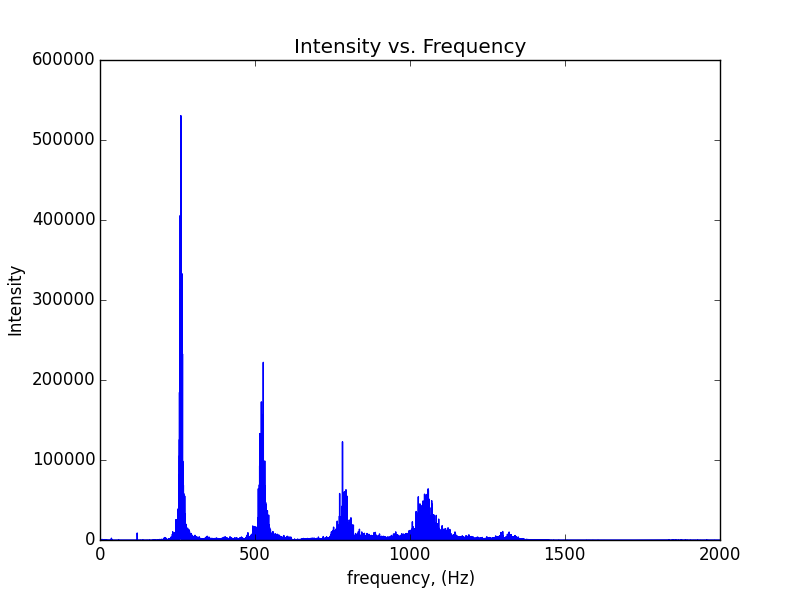
\includegraphics[width=300bp]{noise2_psd.png}
\vspace{-18bp}
\end{center}
\caption[]{\label{fig:psd}\small
Plot of intensity versus frequency. This is the power spectrum distribution
(Fast Fourier Transform and taking magnitude squared) of the data plotted in 
Fig.~\ref{fig:soundvtime}. The peaks in this plot correspond to resonant
frequencies of the tube, which can then be used to calculate the speed of sound.
}
\end{figure}
%------------------------------------------------------------------------------

The next step in the program is to call the function "psd" 
(Power Spectrum Density) from the matplotlib.mlab module. This function is 
passed the mono sound data in the time domain as an array, the total number
of frames, and the sampling rate and returns two arrays corresponding to a 
range of frequencies and their
corresponding intensities. This plot is displayed in Fig.~\ref{fig:psd}.
The peaks in this data therefore correspond to harmonic frequenies that can be
used to calculate the speed of sound in air.

To find the peaks in the transformed data, I added two functions "find\_closest"
and "find\_peaks". The former takes in an array and value and returns the entry
in the array that is closest to the value. The latter uses the first function
to calculate points in the data set that are closest to the expected resonant
frequencies given the physical situation and then iterates through a finite
region of surrounding points to find the maximum in that region. This allows
the program to find multiple extremal points in a noisy data set.

%------------------------------------------------------------------------------
\begin{figure}[h]
\begin{center}
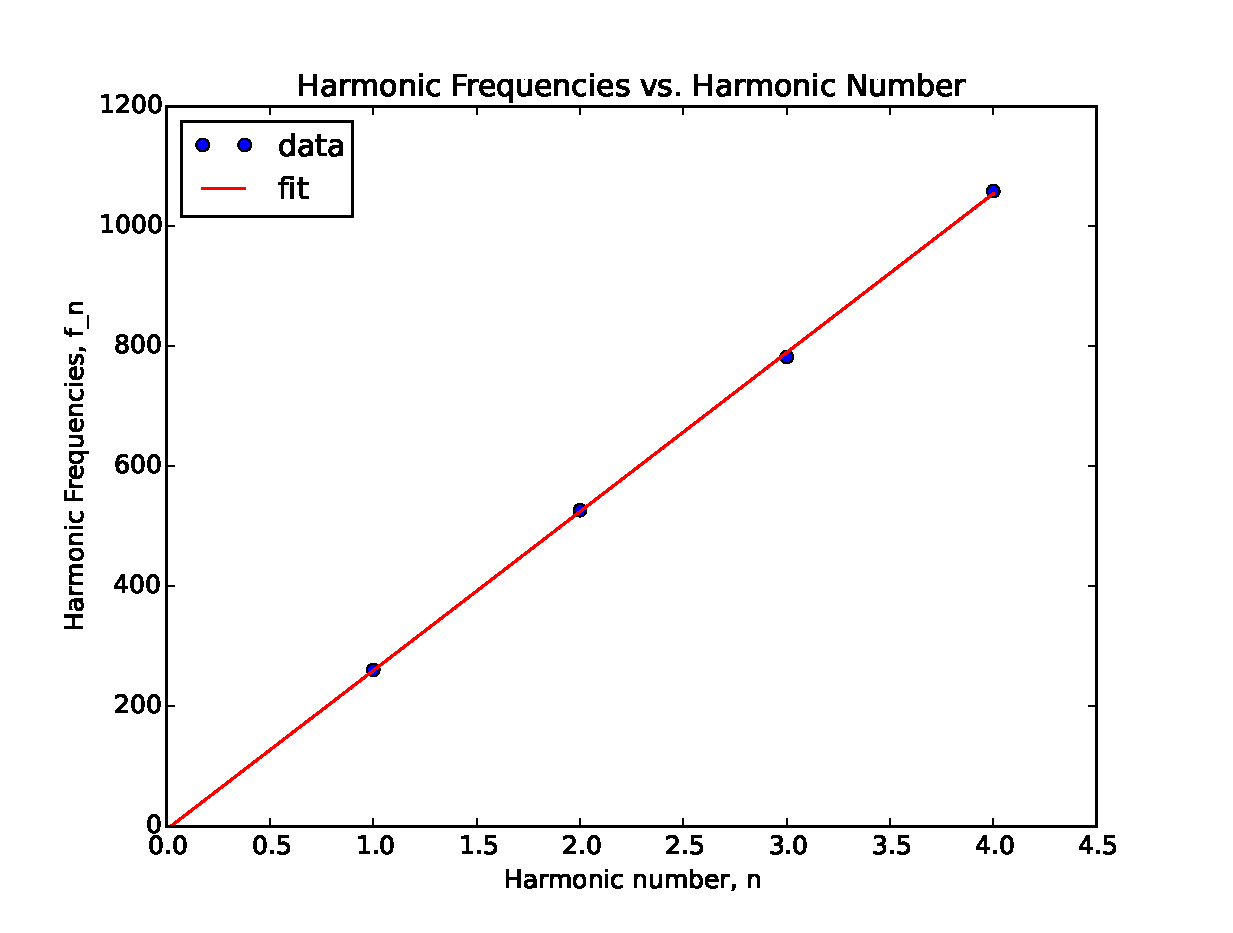
\includegraphics[width=300bp]{noise2_fvn.eps}
\vspace{-18bp}
\end{center}
\caption[]{\label{fig:fvn}\small
Plot of harmonic frequencies versus harmonic number. The resonant frequencies
appear to increase linearly as $n$ incrementally increases, as expected by
the relationship in Eq.~\ref{eq:1}. The slope of this best fit equation is
$264.92 Hz$.
}
\end{figure}
%------------------------------------------------------------------------------

%------------------------------------------------------------------------------
\begin{table}[h]
\begin{center}
\begin{tabular}{ |c|c|c|c|c| }
 \hline
 $n$: & 1 & 2 & 3 & 4 \\
 \hline
 $f_n$ (Hz): & 260.7 & 526.75 & 782.25 & 1058.6 \\
 \hline
\end{tabular}
\end{center}
\caption{Peak frequencies found from data in Fig.~\ref{fig:psd}.}
\label{table:1}
\end{table}
%------------------------------------------------------------------------------
After determining the resonant frequencies, which are tabulated in Table
~\ref{table:1}, the program plots $f_n$ versus $n$ and fits a linear equation 
to the data, as is shown in Fig.~\ref{fig:fvn}. We see from this figure that
the slope of our best fit line is $264.92$ Hz, which, from the relationship 
in Eq.~\ref{eq:1}, must be
$v/2L$. We can thus multiply the slope of our best fit line by $2L$ to obtain
a measurement of the speed of sound in air. This process resulted in a 
measurement of:
\begin{equation} \label{eq:2}
v = 326.35 \quad m/s
\end{equation}
Comparing this to the accepted speed of sound in air of $343$ m/s, we have a
relative error of $4.85\%$.

\end{document}

